\documentclass[a4paper,openright,14pt]{report}
\usepackage[spanish]{babel} % espanol
\usepackage[latin1]{inputenc} % acentos sin codigo
\usepackage{graphicx} % graficos
\usepackage{listings}
\begin{document}

\begin{titlepage}

\begin{center}
\vspace*{-1in}
\begin{figure}[htb]
\begin{center}

\includegraphics[width=4cm]{logo}
\end{center}
\end{figure}

\begin{large}

\end{large}
\vspace*{0.2in}
\begin{Large}
\textbf{Talf laboratorio 1-b} \\
\end{Large}


\vspace*{0.3in}
\rule{80mm}{0.1mm}\\
\vspace*{0.1in}
\begin{large}
Integrantes: Norton Irarr\'azabal \\
Profesor: Eric Castillo \\
Fecha: 29 abril 2019
\end{large}
\end{center}

\end{titlepage}

\newpage
\subsection{Introducci\'on}
\begin{itemize}
\item Se generar\'a una gram\'atica utilizando ANTLR la gram\'atica desarrollada se encuentra en el contexto del lenguaje de consulta SQL. Principalmente resuelve tres tipos de sentencias SELECT, UPDATE, DELETE.
\item Para lograrlo se implementaron clausulas como WHERE ORDER BY y palabras claves FROM, ALL, DISTINCT, ASC, DESC.
\item El objetivo del laboratorio es realizar solo el analizador Lexer que genera un token stream. Sin embargo, para poder realizar lo antes mencionado es necesario codificar un parser.
\item Se ponen en pr\'actica los contenidos vistos en clases de teoría respecto a las gramáticas regulares, que se componen por terminales y no terminales.
\item Se utilizaron 21 terminales y 12 no terminales.
\item Las terminales las identificamos como letras min\'usculas y las no terminales como mayúsculas.
\item Se hizo uso de * para indicar si una terminal o no terminal se repite 0 o n veces.
\item Se uso una gram\'atica de contexto libre en que cada regla de producci\'on es de la forma V -\textgreater w.
	\begin{itemize}
	\item Donde V es un s\'imbolo no terminal y w es una cadena de 					terminales y/o no terminales.
	\end{itemize}
\end{itemize}
\begin{figure}[htb]
\begin{center}
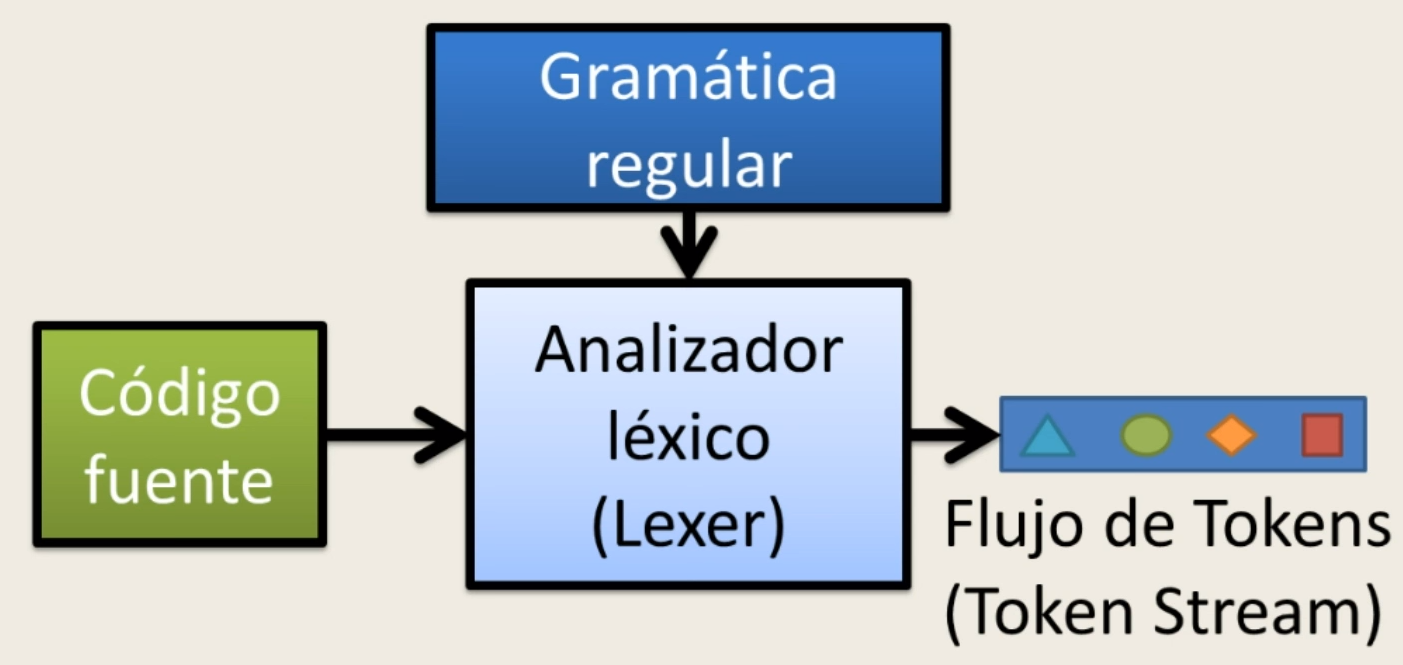
\includegraphics[width=6cm]{imagen10}
\end{center}
\end{figure}
\begin{figure}[htb]
\begin{center}
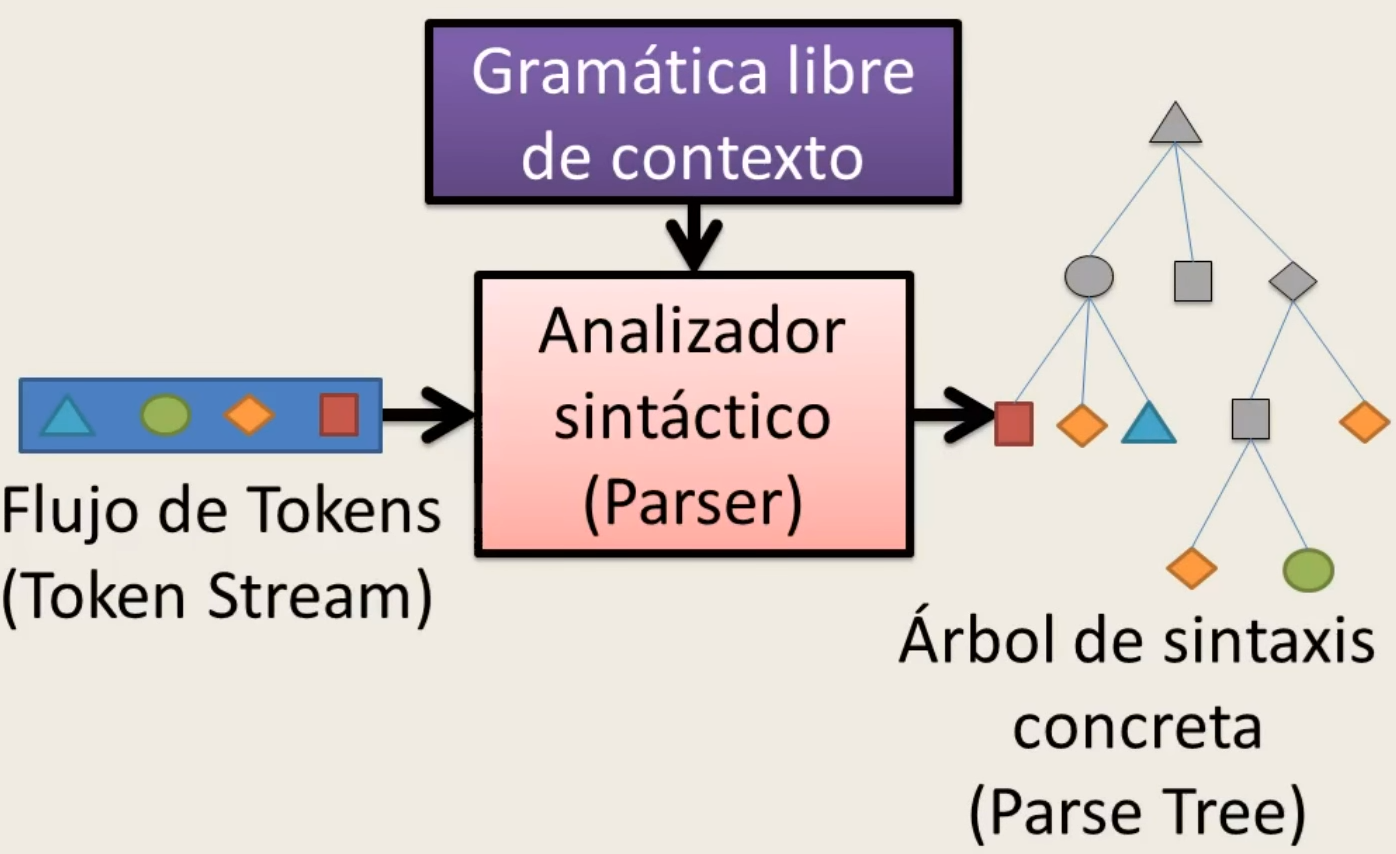
\includegraphics[width=6cm]{imagen12}
\end{center}
\end{figure}




\subsection{Plan general}
\begin{flushleft}
\textbf{Descripci\'on del problema}
\end{flushleft}
\begin{itemize}
\item Generar una gram\'atica utilizando ANTLR.
\end{itemize}
\textbf{\'Ambito}
\begin{itemize}
\item Asignatura de Talf específicamente laboratorio tarea 1-B.
\end{itemize}
\textbf{Alcance}
\begin{itemize}
\item La gram\'atica generada abordara 3 sentencias SQL.
\end{itemize}
\textbf{Restricciones}
\begin{itemize}
\item Lenguaje de programaci\'on java.
\item Software de escritorio.
\item Monousuario.
\item No necesita conexi\'on a internet.
\item Utilizara sistema de control de versiones GitHub.
\end{itemize}
\textbf{Meta}
\begin{itemize}
\item Generar una gram\'atica.
\end{itemize}
\textbf{Objetivos}
\begin{itemize}
\item Instalar, configurar y usar ANTLR.
\item Generar una gram\'atica.
\item Corroborar que la gram\'atica generada funciona.
\item Generar documento similar a manual de usuario.	
\end{itemize}
\subsection{Requerimientos}
\begin{flushleft}
\textbf{Requerimientos funcionales}
\end{flushleft}
\begin{itemize}
\item La gram\'atica debe tener un nombre asignado.
\item Tendr\'a gram\'atica libre de contexto.
\item Tendr\'a gram\'atica regular.
\item Debe funcionar para la gram\'atica SQL espec\'ificamente SELECT, UPDATE, DELETE.
\item La gram\'atica debe funcionar correctamente.
\item La gram\'atica ser\'a probada con 9 consultas.
\begin{lstlisting}
1) SELECT * FROM Coches ORDER BY marca, modelo ASC;
2) SELECT ALL matricula, marca, modelo, color, numero_kilometros, num_plazas 
   FROM Coches
   ORDER BY marca,modelo;
5) SELECT ALL matricula, marca, modelo, color, numero_kilometros, num_plazas
   FROM Coches
   WHERE matricula = 'MF234ZD' OR matricula = 'FK938ZL' ;
6) SELECT ALL matricula,marca, modelo, color, numero_kilometros, num_plazas
   FROM coches 
   WHERE NOT matricula = 'MF-234-ZD';
7) SELECT DISTINCT marca, modelo FROM coches;
8) DELETE FROM tabla WHERE columna1 = 'valor1';
9) UPDATE My_table SET field1 = 'a' WHERE field2 = 'N';
\end{lstlisting}
\begin{itemize}
\item Se debe visualizar vista de la gram\'atica.
\end{itemize}
\textbf{Requerimientos no funcionales}
\begin{itemize}
\item Sera monousuario.
\item Debe ser capaz de ejecutarse en no m\'as de 4 seg.
\item Debe proporcionar mensajes de error en caso de que ocurran.
\item El software debe contar con manual de usuario.
\item No se tomar\'a en cuenta la seguridad.
\item Se utilizar\'a nomenclatura snake\_case.
\item No debe ser complejo de usar.
\item Utilizar\'a lenguaje de programaci\'on java.
\item Har\'a uso de ANTLR.
\item Sera de escritorio.
\end{itemize}	
\end{itemize}
\subsection{ANTLR}
Herramienta que opera sobre lenguajes, proporcionando un marco para construir reconocedores (parsers), int\'erpretes, compiladores y traductores de lenguajes a partir de las descripciones gramaticales de los mismos.\\\\
Partiendo de la descripci\'on formal de la gram\'atica de un lenguaje, ANTLR genera un programa que determina si una sentencia o palabra pertenece a dicho lenguaje (reconocedor). Si a dicha gram\'atica, se le a\~naden acciones escritas en un lenguaje de programaci\'on, el reconocedor se transforma en un traductor o int\'erprete.\\\\
Disponible para:  Linux, Windows y Mac OS X. \\
Inicio: A\~no 1988.\\
Versi\'on actual: 4.7.2.\\
Se hace uso de ANTLR en: Twitter, Pig Hive, Hadoop, Lex Machina, Oracle, NetBeans, Lenguaje HQL.
\subsection{Manual de usuario}
\begin{itemize}
\item \textbf{Instalaciones previas} 
\item JDK 12
\end{itemize}
\begin{figure}[htb]
\begin{center}
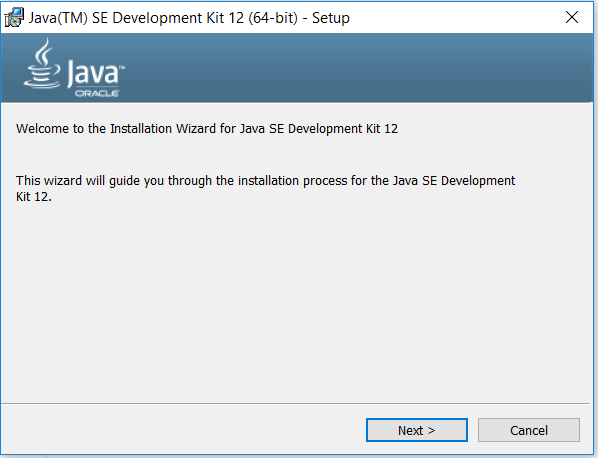
\includegraphics[width=10.3cm]{imagen2}
\end{center}
\end{figure}
\begin{itemize}
\item JRE 1.8
\end{itemize}
\begin{figure}[htb]
\begin{center}
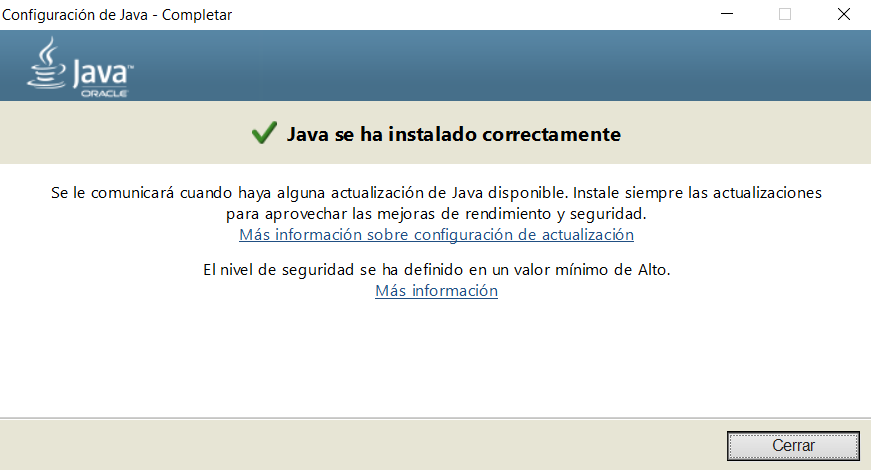
\includegraphics[width=9.2cm]{imagen3}
\end{center}
\end{figure}
\newpage
\begin{itemize}
\item Eclipse jee-2019-0
\end{itemize}
\begin{figure}[htb]
\begin{center}
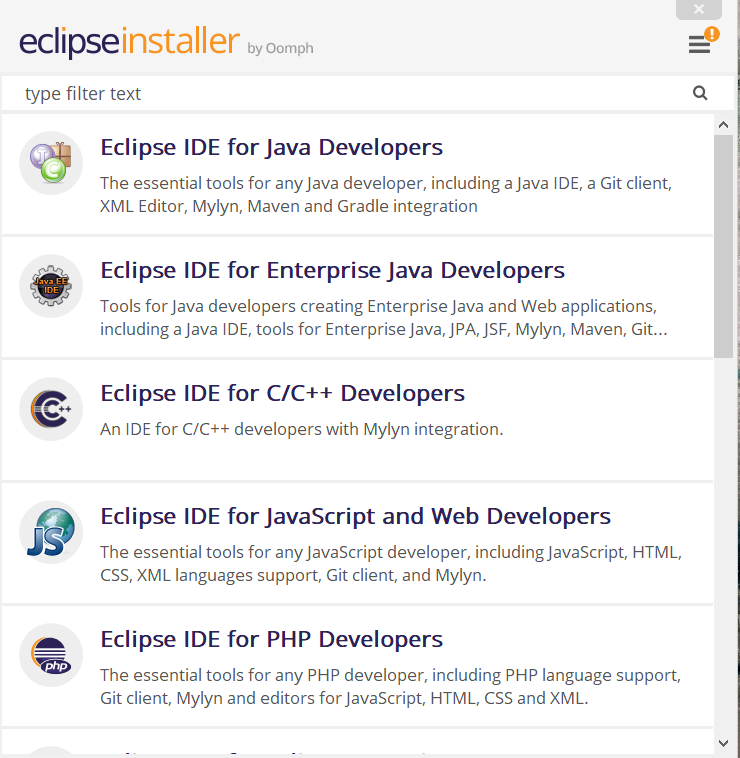
\includegraphics[width=9.2cm]{imagen4}
\end{center}
\end{figure}
\newpage
\begin{itemize}
\item Instalaci\'on de ANTLR
\end{itemize}
\begin{figure}[htb]
\begin{center}
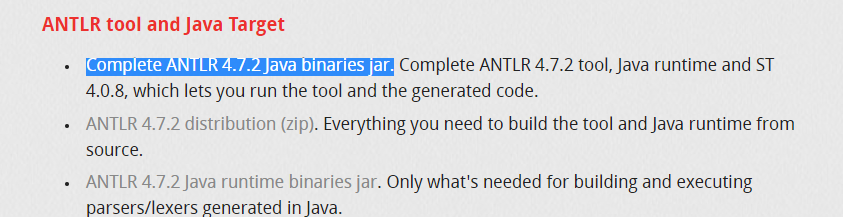
\includegraphics[width=9.2cm]{imagen5}
\end{center}
\end{figure}
\begin{figure}[htb]
\begin{center}
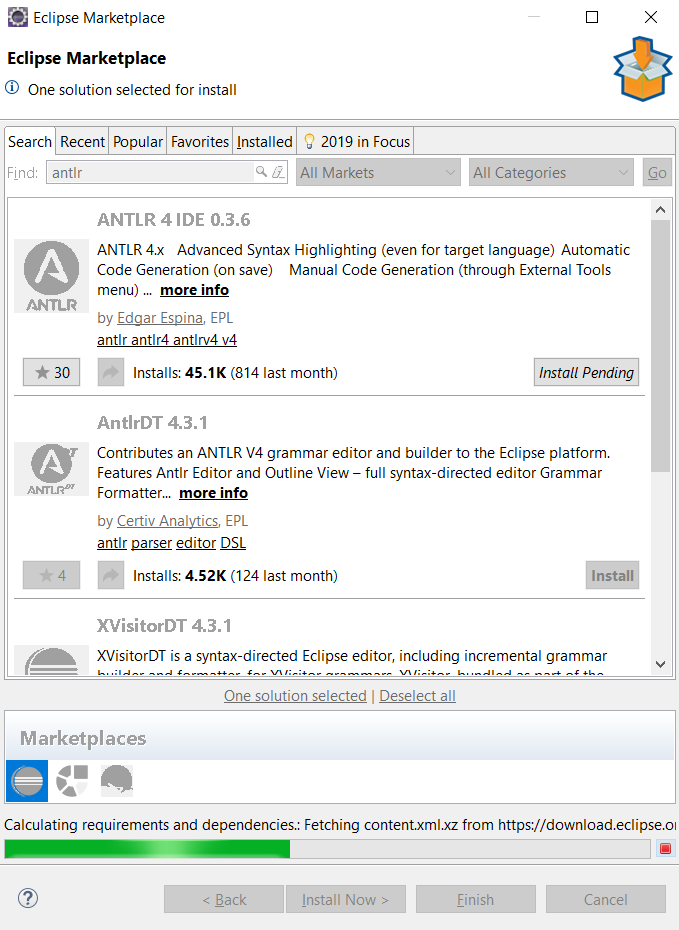
\includegraphics[width=9cm]{imagen6}
\end{center}
\end{figure}
\newpage
\begin{figure}[htb]
\begin{center}
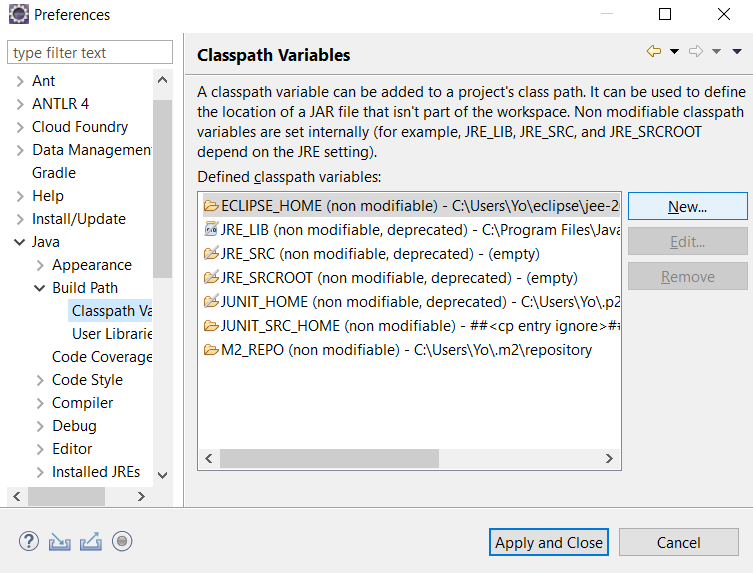
\includegraphics[width=9.2cm]{imagen7}
\end{center}
\end{figure}
\begin{figure}[htb]
\begin{center}
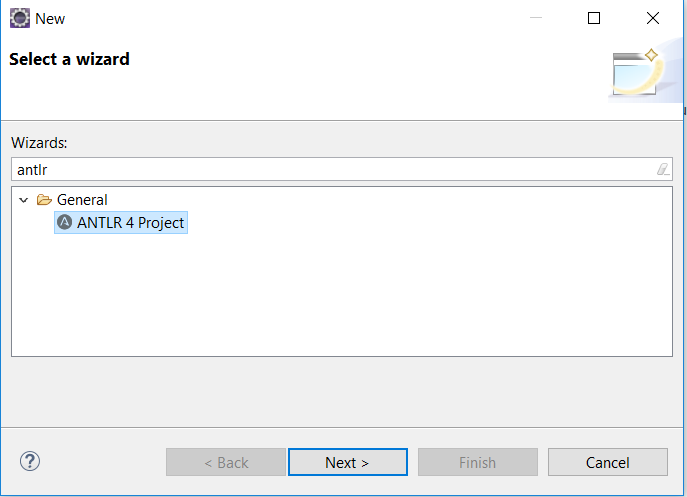
\includegraphics[width=9.2cm]{imagen8}
\end{center}
\end{figure}
\newpage
\begin{figure}[htb]
\begin{center}
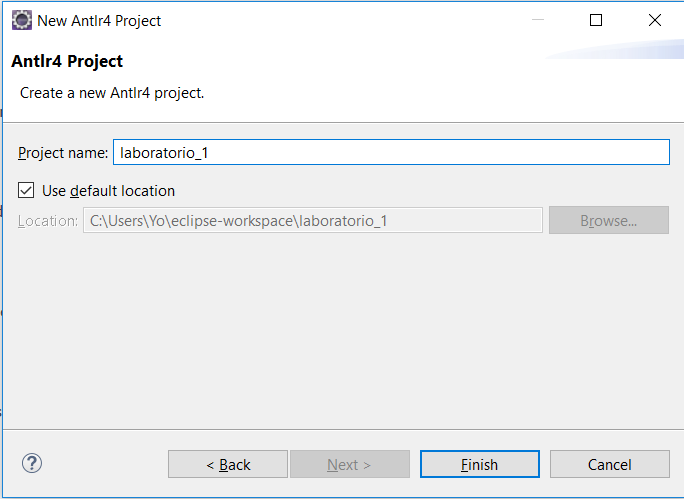
\includegraphics[width=9.2cm]{imagen9}
\end{center}
\end{figure}
\newpage
\subsection{C\'odigo}
\begin{itemize}
\item \textbf{No terminales}
\end{itemize}
\begin{lstlisting}
consulta: (select | update | delete);

select: SELECT (ASTERISCO| ( (ALL | DISTINCT) (nombre_de_campo_coma* ID))) from;
update: UPDATE ID SET condicion_coma* condicion where;
delete: DELETE from;

from: FROM ID (PUNTO_COMA | order_by | where);

order_by: ORDER_BY nombre_de_campo_coma* condicion_asc_desc; 
where: WHERE NOT* condicion_AND_OR* condicion PUNTO_COMA;

condicion_asc_desc: ID (ASC|DESC) PUNTO_COMA;
nombre_de_campo_coma: ID COMA;

condicion_AND_OR: condicion (AND|OR);
condicion_coma: condicion COMA;
condicion: ID IGUAL COMILLA ID COMILLA;
\end{lstlisting}
\begin{itemize}
\item \textbf{Terminales}
\end{itemize}
\begin{lstlisting}
SELECT:'SELECT';
DELETE:'DELETE';
UPDATE:'UPDATE';

ALL:'ALL';
DISTINCT:'DISTINCT';

FROM:'FROM';
WHERE:'WHERE';
NOT:'NOT';

OR:'OR';
AND:'AND';

SET:'SET';
ASC:'ASC';
DESC:'DESC';
ID: [a-zA-Z_][a-zA-Z0-9_\-]*;

ORDER_BY:'ORDER BY';

PUNTO_COMA:';';

ASTERISCO:'*';

COMA:',';

IGUAL:'=';
COMILLA :'\'';

WS: [ \t\n\r]+ -> skip;
\end{lstlisting}
\subsection{Siga los siguientes pasos para ver gram\'atica}
\begin{figure}[htb]
\begin{center}
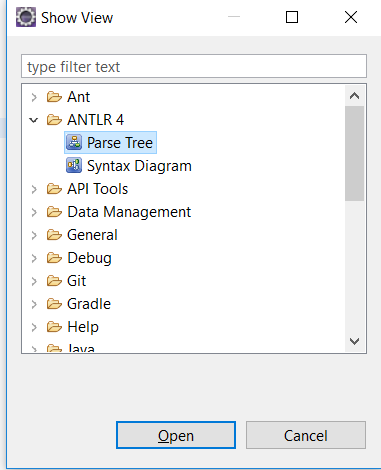
\includegraphics[width=9.2cm]{imagen14}
\end{center}
\end{figure}
\begin{figure}[htb]
\begin{center}
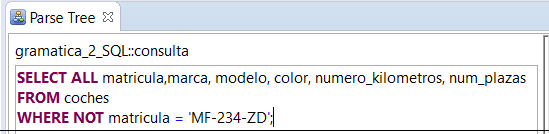
\includegraphics[width=9.2cm]{imagen15}
\end{center}
\end{figure}
\newpage
\begin{figure}[htb]
\begin{center}
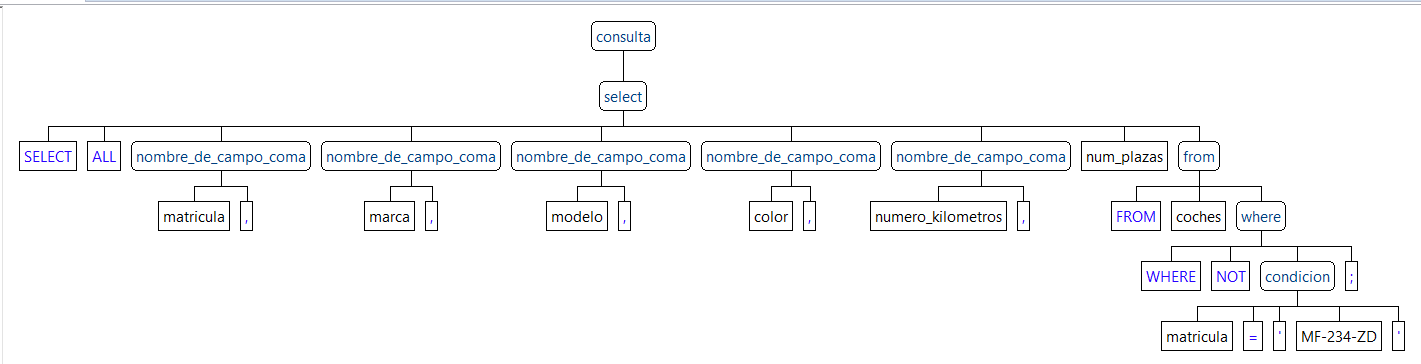
\includegraphics[width=15cm]{imagen16}
\end{center}
\end{figure}
\end{document}